\begin{surferPage}[Kummer-Quartic]{The Kummer Quartic}
    In 1875, Eduard Kummer was the first person who explicitly asked the question
    of what the maximum number $\mu(d)$ of singularities on a surface of degree
    $d$ are. In his case the degree was $4$ and are called \emph{quartics}. 
  
  He showed that $\mu(4)=16$. After that he studied quartics with $16$
    singularities in detail.
    A particularly beautiful family of such surfaces is given by:
    \[\bigl(x^2+y^2+z^2-\mu^2\bigr)^2 - \lambda
    \,y_0\,y_1\,y_2\,y_3,\]
    where $\mu$ is a free parameter, and 
    $\lambda = \frac{3\mu^2-1}{3-\mu^2}$; the $y_i$ are the sides of a regular
    tetrahedron {\small
    $y_0=1-z-\sqrt{2}x$, \  
    $y_1=1-z+\sqrt{2}x$, \ 
    $y_2=1+z+\sqrt{2}y$, \ 
    $y_3=1+z-\sqrt{2}y$}
  in order to make the surface symmetric.
  Not all members of this family have exactly $16$ real singularities,
  although most of them do:
  \begin{center}
    \vspace*{-0.2cm}\hspace*{-0.2cm}
    \begin{tabular}{@{}c@{\,}c@{\,}c@{\,}c@{\,}c@{}}
      \begin{tabular}{@{}c@{}}
        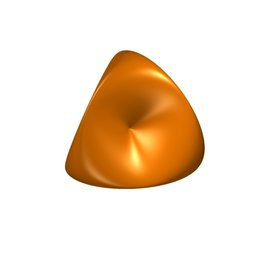
\includegraphics[height=1.4cm]{kummer_0}
      \end{tabular}
      &
      \begin{tabular}{@{}c@{}}
        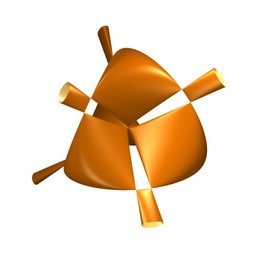
\includegraphics[height=1.4cm]{kummer_1}
      \end{tabular}
      &
      \begin{tabular}{@{}c@{}}
        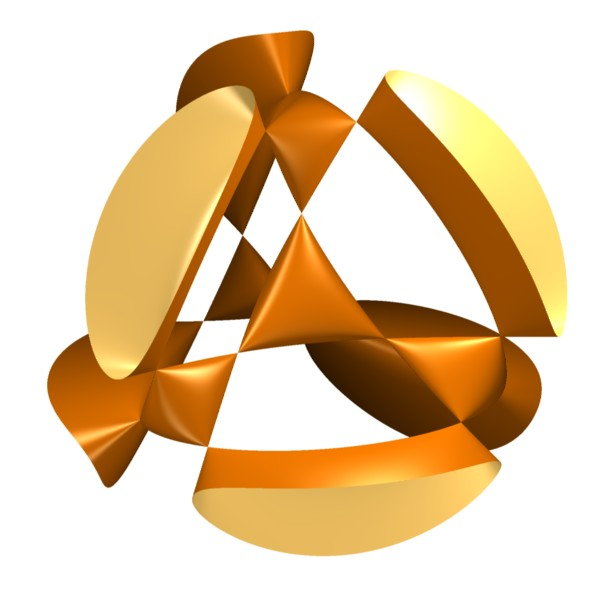
\includegraphics[height=1.4cm]{kummer_2}
      \end{tabular}
      &
      \begin{tabular}{@{}c@{}}
        
\includegraphics[height=1.4cm]{kummer_3}
      \end{tabular}
    \end{tabular}
  \end{center}
  \vspace{-0.2cm}  
   For some special values of the parameters, several of the singularities may
  coincide.
\end{surferPage}
